\documentclass{article}
\usepackage{graphicx}
\usepackage{graphics}
\graphicspath{{/home/user/images/},{/home/personnels/berhe/TextClassification/}}
\usepackage{amsmath}
\usepackage{fancyhdr}

\setlength{\parindent}{0em}
\setlength{\parskip}{1em}
\renewcommand{\baselinestretch}{1.5}

\pagestyle{fancy}
\fancyhf{}
\rfoot{Page \thepage}
\lfoot{text classification}

\title{Text Classification }
\title{Data Visualization on Pompe Diseases}
\author{Aman Berhe}

\begin{document}
\maketitle
\newpage
The Dimention of the Positive and negative words: 
\begin{table}[h!]
  \centering
  \caption{Pompe Diseases with all the words and total number of sentences }
  \label{tab:table1}
  \begin{tabular}{l|c c c c|r}
      Pompe data  & positive & negative & vector& \\
    \hline
      Words & 2663 & 11029 & 3& \\
    \hline
      sentence & 69 & 416 & 1& \\
  \end{tabular}
\end{table}
\begin{table}[h!]
  \centering
  \caption{Pompe Diseases with punctuation removed words in a sentence and total number of sentences }
  \label{tab:table1}
  \begin{tabular}{l|c c c c|r}
      Pompe data  & positive & negative & vector& \\
    \hline
      Words & 2155 & 9684  & 3& \\
    \hline
      sentence & 69 & 416 & 1& \\
  \end{tabular}
\end{table}
\begin{table}[h!]
  \centering
  \caption{Pompe Diseases with punctuation removed words in a sentence and total number of sentences }
  \label{tab:table1}
  \begin{tabular}{l|c c c c|r}
      Pompe data  & positive & negative & vector& \\
    \hline
      Words & 1789 & 8138  & 3& \\
    \hline
      sentence & 69 & 416 & 1& \\
  \end{tabular}
\end{table}
\newpage
Here are some pictures which shows the occurrence of words. the words satisfy the Zipf's Law\\
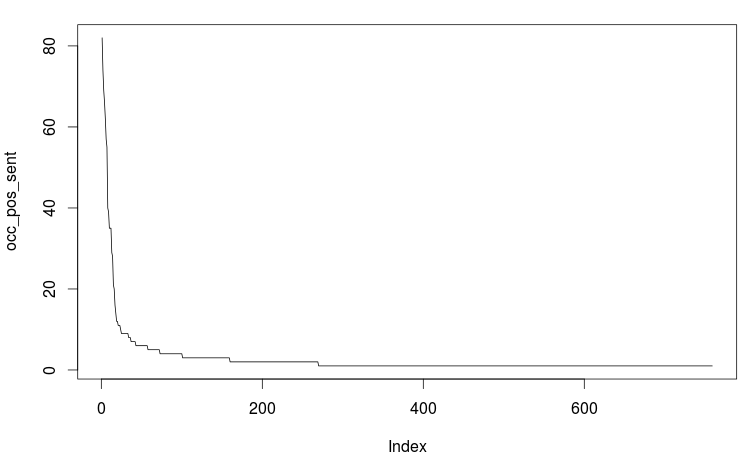
\includegraphics[width=0.7\linewidth]{visual1.png}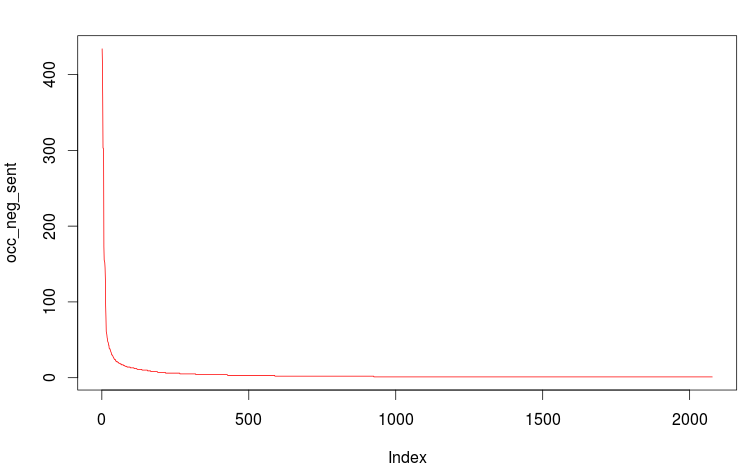
\includegraphics[width=0.7\linewidth]{visual2.png}\\
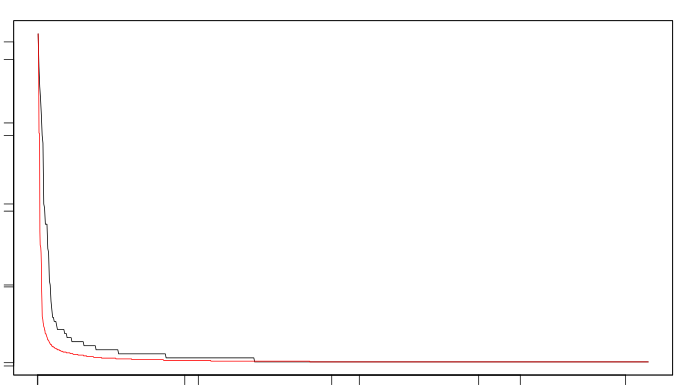
\includegraphics[width=0.9\linewidth]{visual1and2.png}\\

The More the data the curve is very smooth. The curves of the unique words in a sentence is very similar to the above pictures

\newpage
Plots of Word frequency: here I take only one word per sentence\\
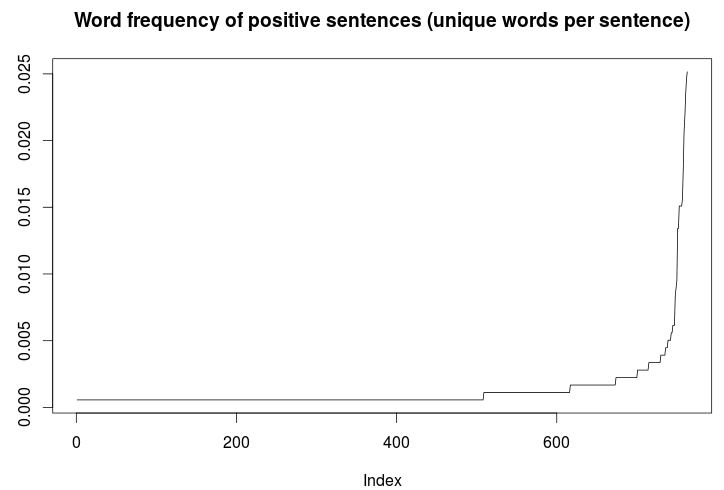
\includegraphics[width=0.9\linewidth]{Word_frequency_pos.png}\\
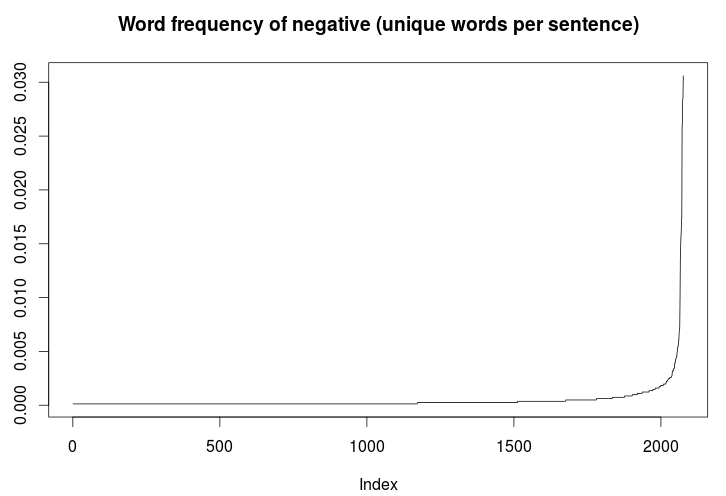
\includegraphics[width=0.9\linewidth]{Word_frequency_neg.png}\\

The plots of word frequency and unique word per sentence occurrence look almost alike since the occurrence is used to compute the frequency
\newpage
Here are the top 20 words\\
for all words in a snetence\\
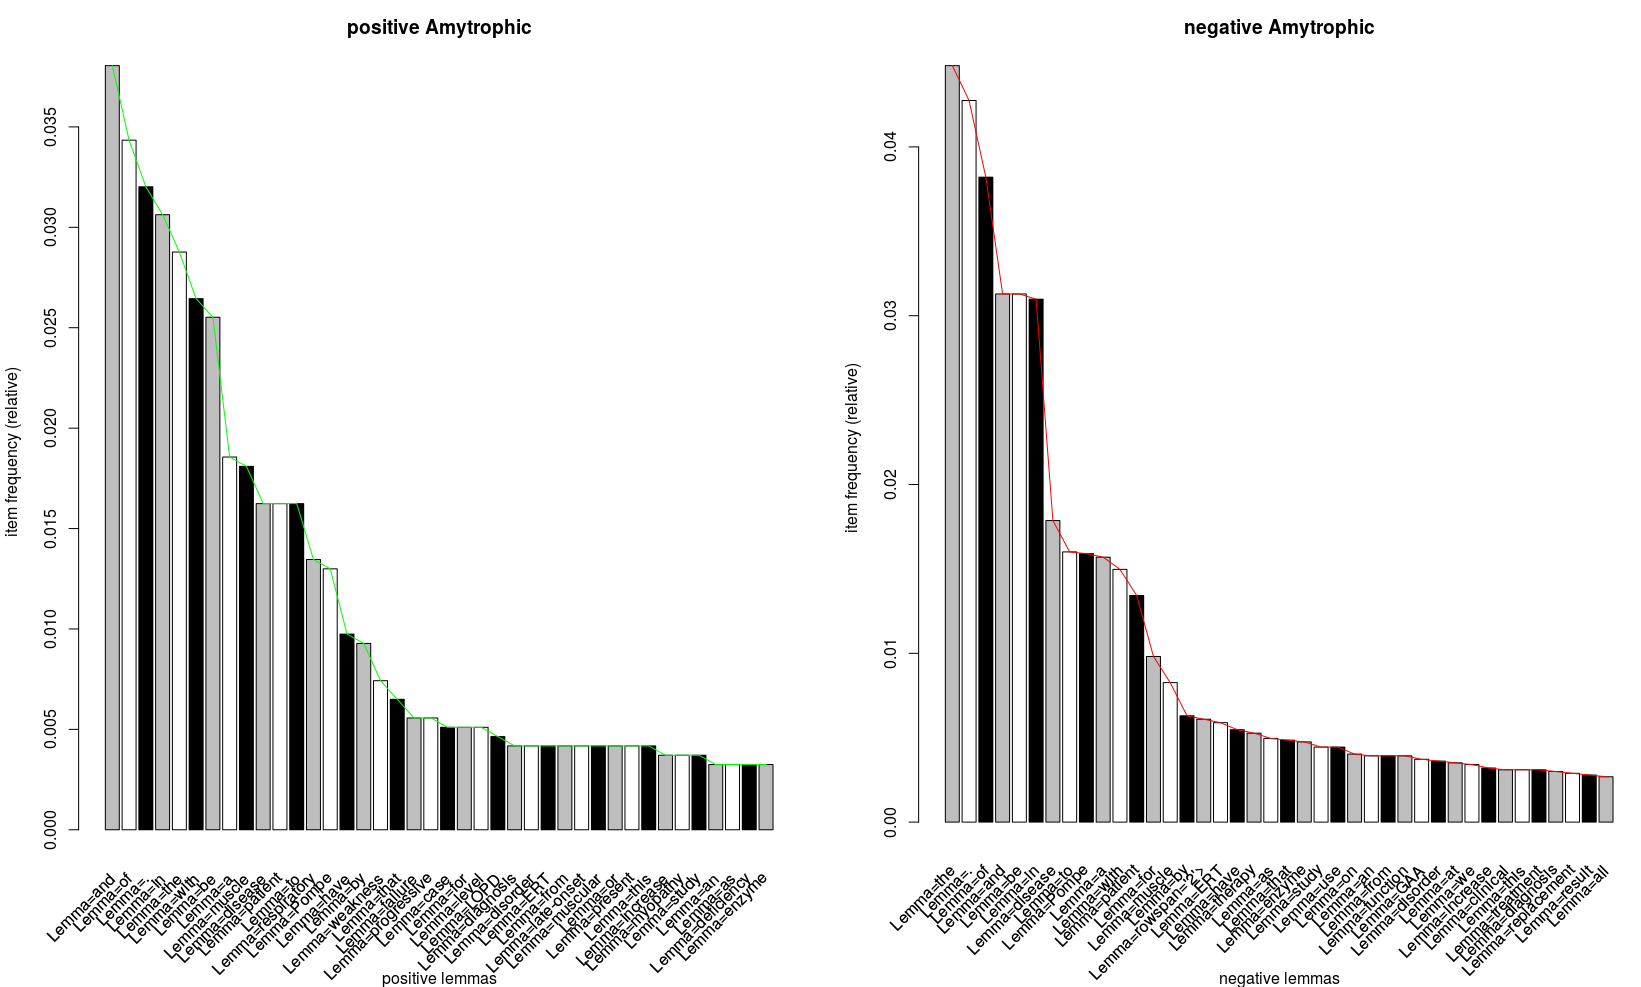
\includegraphics[width=1.0\linewidth]{Top_20_lemma.png}\\
for the unque words per sentence\\
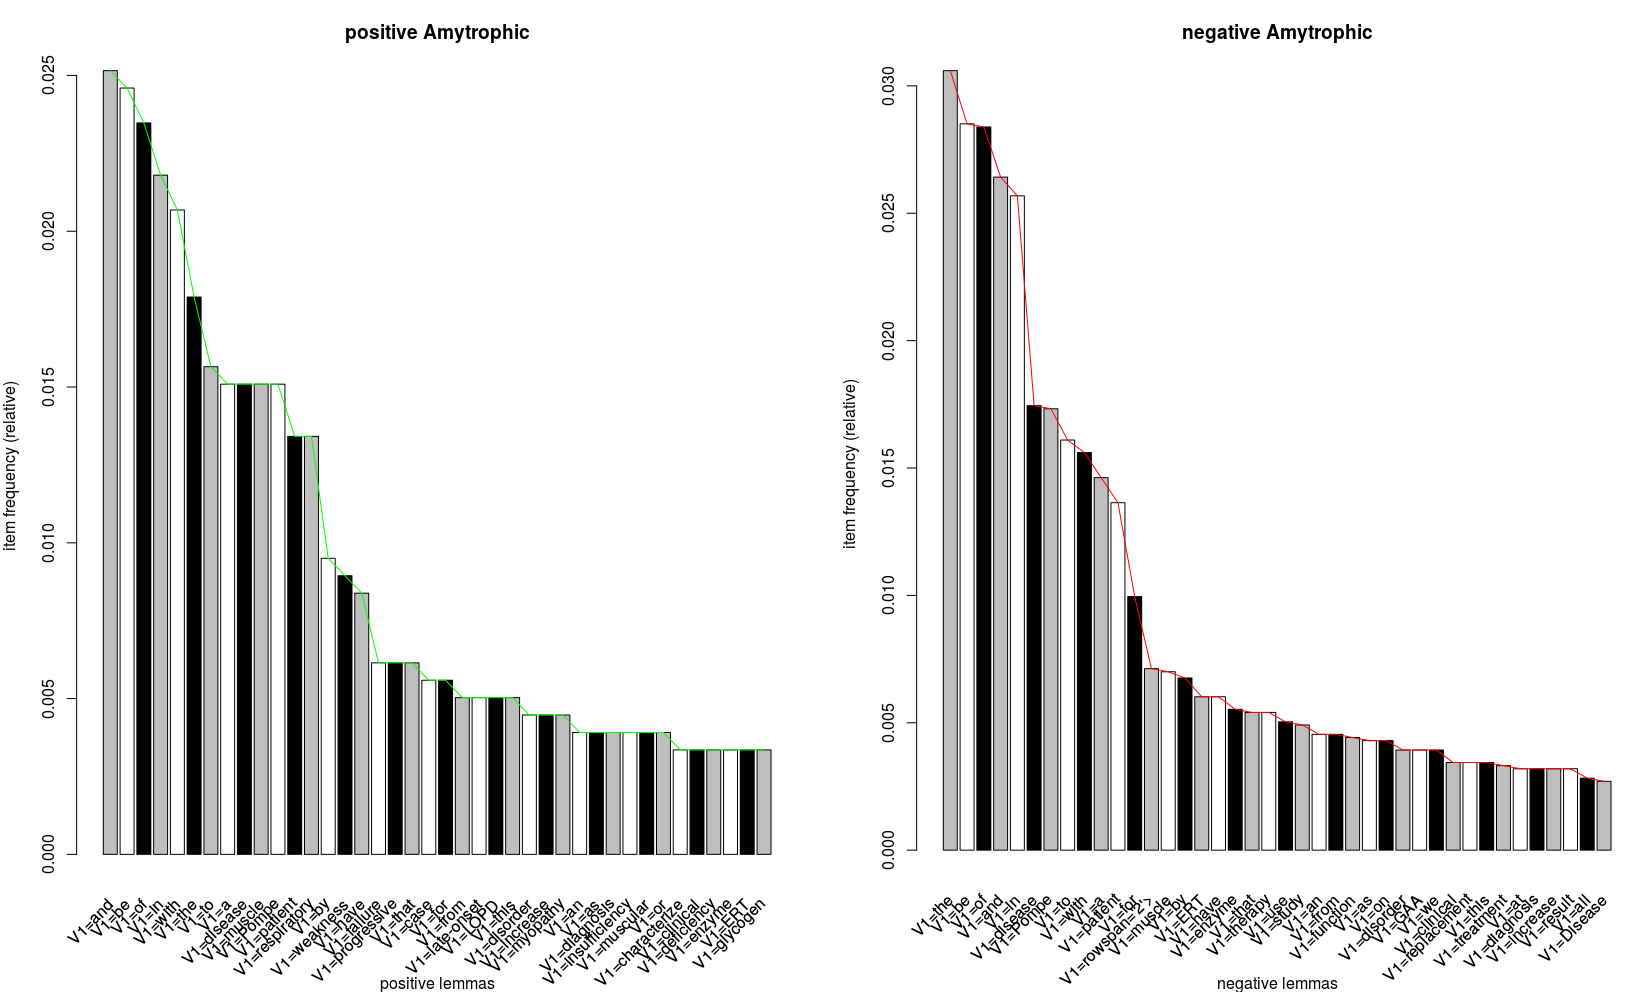
\includegraphics[width=1.0\linewidth]{Top_20_lemma_uniq.png}\\
The following shows the gross rate of the words on total number of words \\
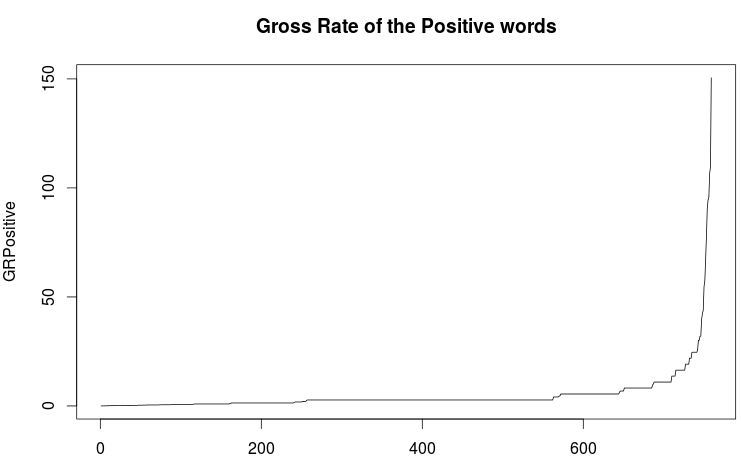
\includegraphics[width=0.6\linewidth]{vis_GR.png}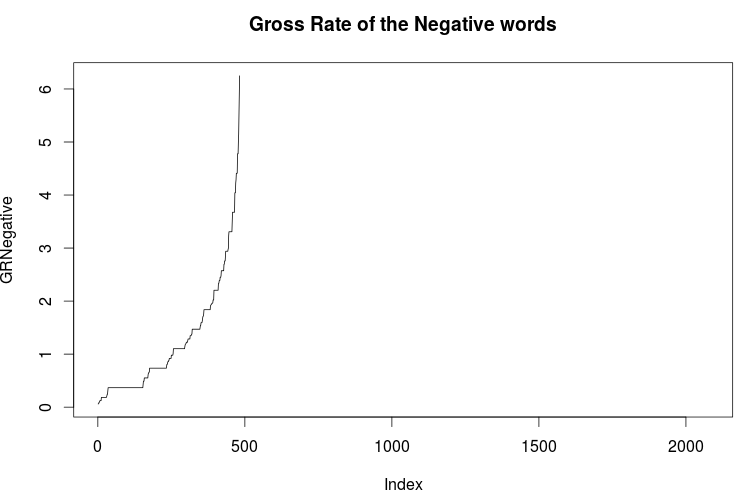
\includegraphics[width=0.6\linewidth]{vis_GR3.png}\\
The following shows the gross rate of the unique words in a sentence on total number of words\\
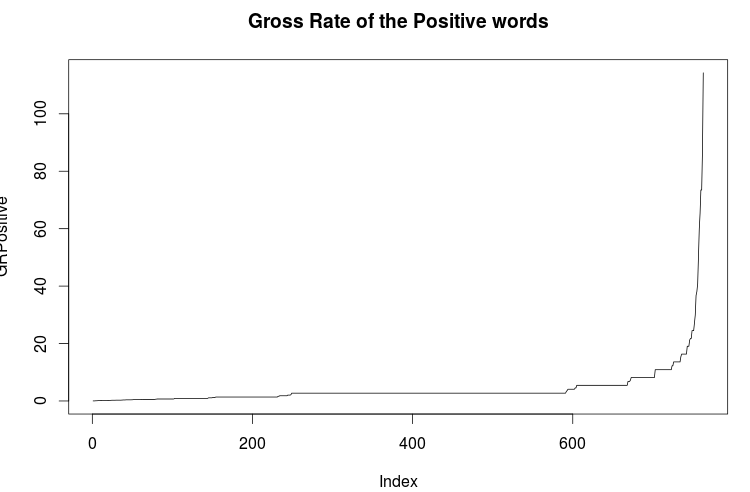
\includegraphics[width=0.6\linewidth]{vis_GR2.png}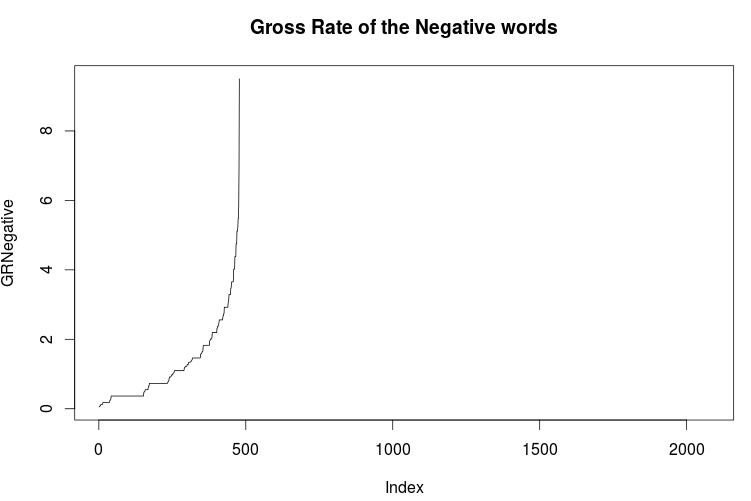
\includegraphics[width=0.6\linewidth]{vis_GR4.png}\\
comparison between the unique words per sentence and total words in a \\
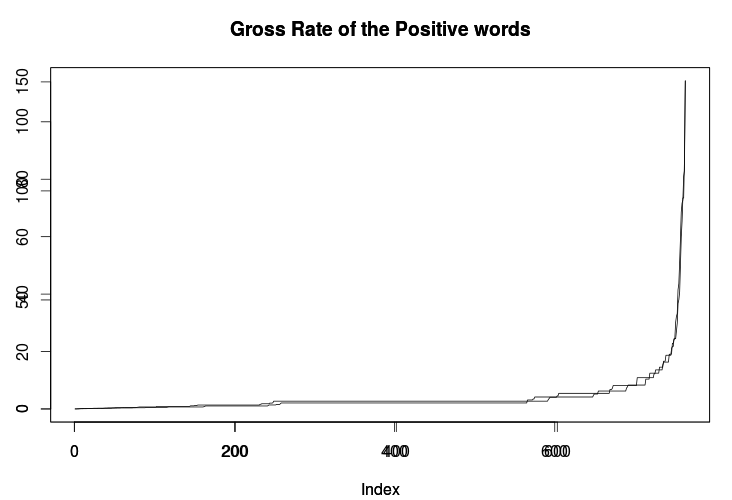
\includegraphics[width=0.7\linewidth]{vis_GR_pos.png}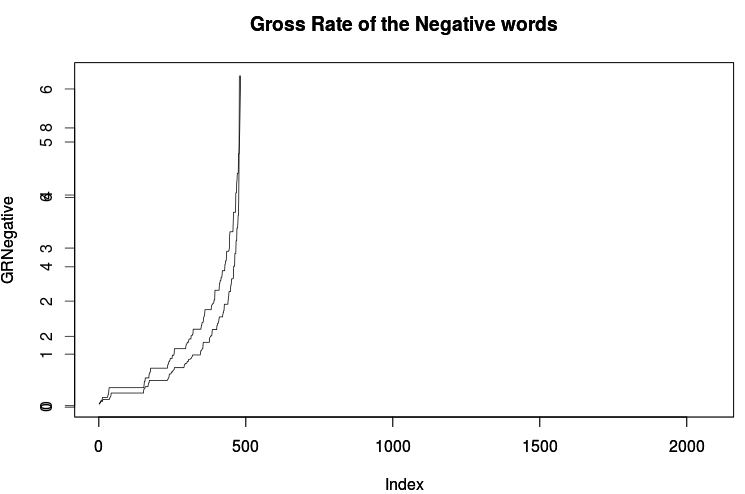
\includegraphics[width=0.7\linewidth]{vis_GR_neg.png}\\

The following shows the gross rate of the words over total number sentences \\
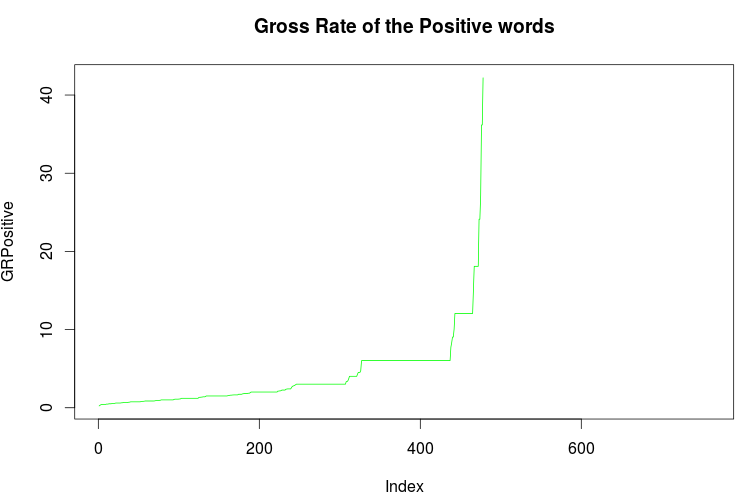
\includegraphics[width=0.7\linewidth]{vic_GR_sent_pos.png}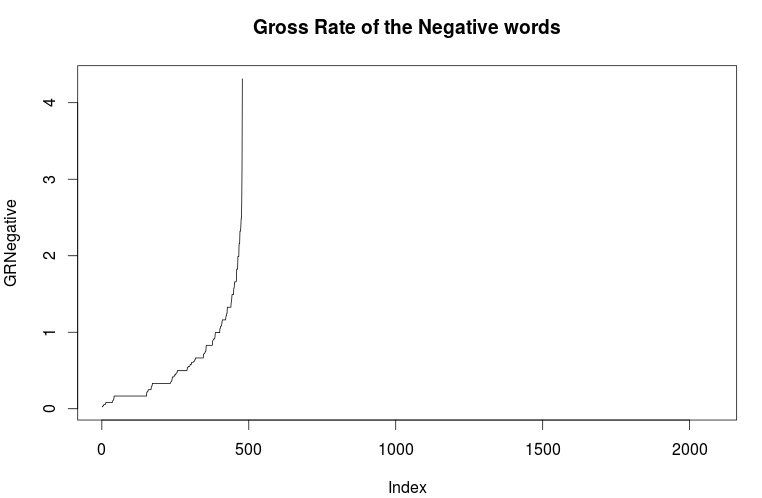
\includegraphics[width=0.7\linewidth]{vic_GR_sent_neg.png}\\
TF-IDF representation of the words look like this\\
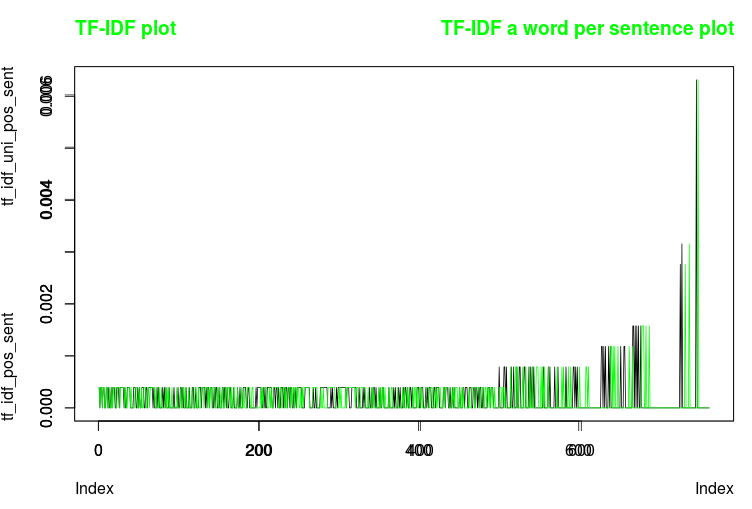
\includegraphics[width=0.7\linewidth]{TF_IDF_pos.png}\\
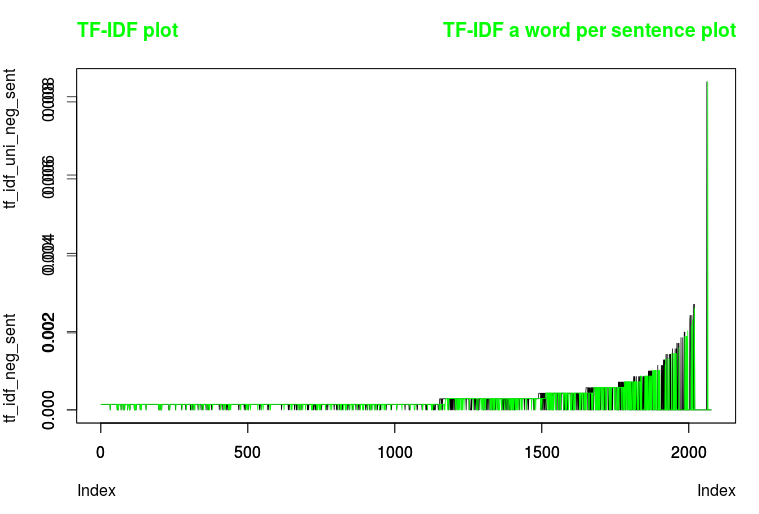
\includegraphics[width=0.7\linewidth]{TF_IDF_neg.png}\\
The Tf-IDF is computed by: if the word exists in both documents it will be $0$ if not its frequency will be multiplied by 0.3 $(\log(2))$

 {\LARGE \textbf {Words and their Occurrence}}\\
 The words and their ocuurence has benn put side by side like this\\
 positive data\\
 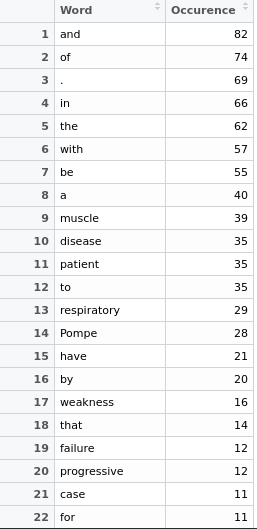
\includegraphics[width=0.6\linewidth]{word_occurence_pos.png}
 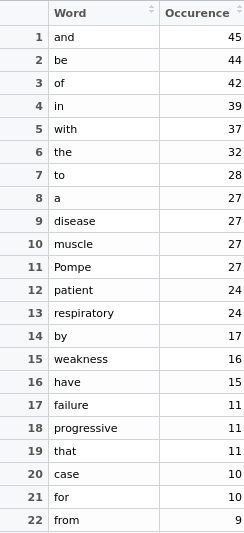
\includegraphics[width=0.6\linewidth]{word_occurence_pos_uni.png}\\
 
 \newpage
negative data\\
 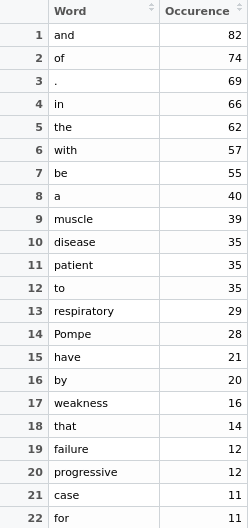
\includegraphics[width=0.6\linewidth]{word_occurence_neg.png}
 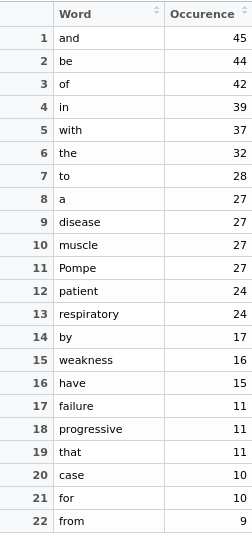
\includegraphics[width=0.6\linewidth]{word_occurence_neg_uni.png}\\
 
 {\LARGE \textbf {Removed Stop Words}}\\
 words with greater than 40 occurrence has been removed and the result is as follows 
  positive data\\
  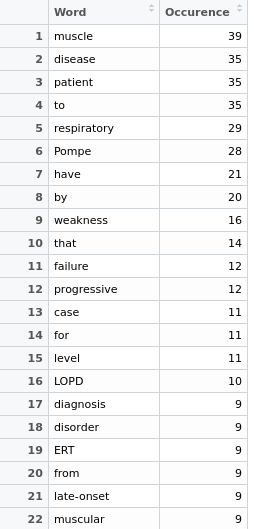
\includegraphics[width=0.6\linewidth]{Rem_stop_words.png}
  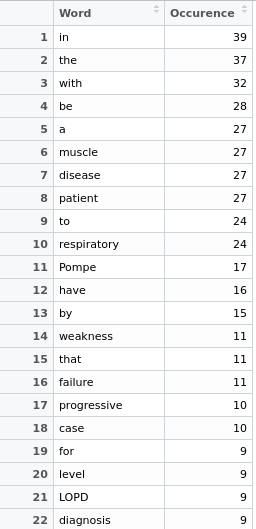
\includegraphics[width=0.6\linewidth]{Rem_stop_words_uni.png}\\
  positive data\\
    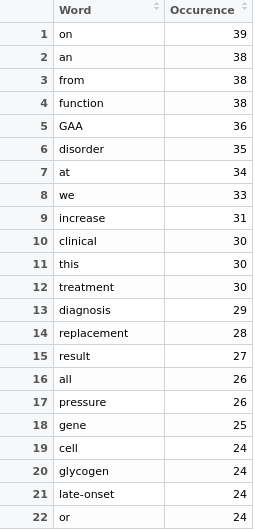
\includegraphics[width=0.6\linewidth]{Rem_stop_words_neg.png}
    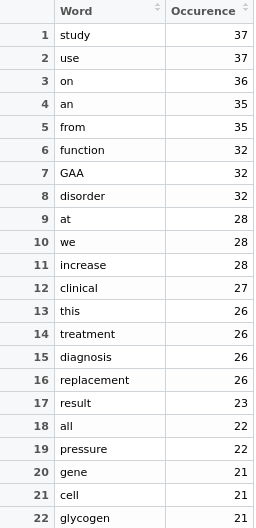
\includegraphics[width=0.6\linewidth]{Rem_stop_words_uni_neg.png}\\
\end{document}